\documentclass[11pt]{article}
\usepackage[margin=1in]{geometry}
\usepackage{amsmath,amssymb,amsthm,mathtools}
\usepackage{graphicx}
\usepackage{microtype}
\usepackage[hidelinks]{hyperref}
\usepackage{enumitem}

\newtheorem{theorem}{Theorem}
\newtheorem{lemma}{Lemma}
\newtheorem{remark}{Remark}
\newcommand{\C}{\mathbb C}
\newcommand{\R}{\mathbb R}
\newcommand{\U}{\mathcal U}
\newcommand{\diag}{\operatorname{diag}}
\newcommand{\conv}{\operatorname{conv}}

\title{Exact Continuous Majorization on the Simple-Spectrum Stratum}
\author{Candidate partial result for arXiv:2210.13309}
\date{26 August 2026}

\begin{document}
\maketitle

\begin{center}
\fbox{\parbox{0.91\textwidth}{\textbf{Status.}
Candidate partial result, likely valid, pending human review.  Question 7.2 of
the source has an affirmative answer whenever the majorizing field has simple
spectrum at every point.  In that case the desired element is the average of
exactly $n$ continuous unitary conjugates, with all weights equal to $1/n$.
The argument does not treat eigenvalue collisions.}}
\end{center}

\section{Source question}

Mootoo and Skoufranis study several versions of joint majorization in
$C(X,M_n(\C))$ and show that pointwise majorization characterizes the
\emph{closed} convex hull of a joint unitary orbit \cite{MS}.  Their Question
7.2 asks whether closure can be removed for one self-adjoint operator:
\begin{quote}
Let $A,B\in C(X,M_n)$ be self-adjoint and continuously diagonalizable.  Does
$A\prec_c B$ imply that $A\in\conv(\U(B))$?
\end{quote}

\begin{figure}[ht]
\centering
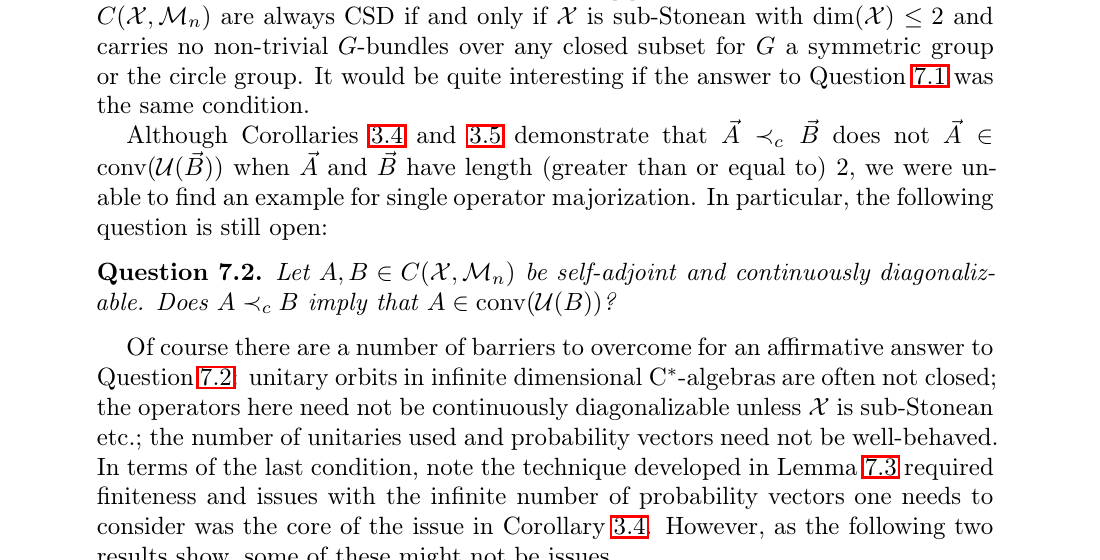
\includegraphics[width=0.96\textwidth]{source_question_crop.png}
\caption{Question 7.2 in the published source, page 20.}
\end{figure}

Here $A\prec_c B$ means that, after continuous diagonalizations, a continuous
doubly stochastic matrix field sends the eigenvalue vector of $B$ to that of
$A$.  The conclusion $A\in\conv(\U(B))$ requires one finite probability vector,
independent of $x\in X$, and continuous unitary fields.

\section{Result}

\begin{theorem}[Simple-spectrum affirmative answer]\label{thm:main}
Let $X$ be a compact Hausdorff space, and let $A,B\in C(X,M_n(\C))$ be
self-adjoint and continuously diagonalizable.  Assume that $A\prec_c B$ and
that $B(x)$ has simple spectrum for every $x\in X$.  Then there exist unitaries
$U_0,\ldots,U_{n-1}\in C(X,M_n(\C))$ such that
\[
             A=\frac1n\sum_{k=0}^{n-1}U_k^*BU_k.
\]
In particular, $A\in\conv(\U(B))$, with $n$ equal weights.
\end{theorem}

The conclusion is stronger than merely showing that $A$ belongs to an
unspecified finite convex hull.  It provides a number of summands depending
only on the matrix size and a fixed probability vector.

\section{Idea of the proof}

For a strictly ordered vector $b=(b_1,\ldots,b_n)$, the possible diagonals of
the Hermitian orbit of $D_b=\diag(b)$ form the permutahedron
\[
                    P(b)=\conv\{\sigma b:\sigma\in S_n\}.
\]
The Schur--Horn theorem gives surjectivity of the diagonal map onto $P(b)$,
but a pointwise choice of a conjugating unitary is not enough here: it must
vary continuously with both $a$ and $b$.

The key observation is that a single compact slice works simultaneously for
all strictly ordered $b$.  Take the closure of a generic diagonal-torus orbit
in the full flag variety.  This is the permutohedral toric variety, and its
nonnegative part maps homeomorphically to $P(b)$ under the $b$-weighted moment
map.  That nonnegative part is contractible, so its flag bundle admits a
continuous unitary lift.  We thereby obtain a jointly continuous unitary
$R(a,b)$ for which
\[
             \diag\bigl(R(a,b)D_bR(a,b)^*\bigr)=a.
\]
Finally, averaging this matrix over the $n$ cyclic diagonal phase matrices
kills every off-diagonal entry without changing its diagonal.  Each summand
remains a unitary conjugate of $D_b$.

\section{A uniform toric Schur--Horn slice}

Let
\[
       \mathcal C=\{b\in\R^n:b_1>b_2>\cdots>b_n\}.
\]

\begin{lemma}[Uniform slice]\label{lem:slice}
There are a compact contractible space $T_n$ and a continuous map
$R:T_n\to U(n)$ such that, for every $b\in\mathcal C$, the map
\[
 \theta_b:T_n\longrightarrow P(b),\qquad
 \theta_b(t)=\diag\bigl(R(t)D_bR(t)^*\bigr),
\]
is a homeomorphism.  Moreover, for every compact $K\subset\mathcal C$, the
inverse
\[
 \{(b,a):b\in K,\ a\in P(b)\}\longrightarrow T_n,
 \qquad (b,a)\longmapsto\theta_b^{-1}(a)
\]
is continuous.
\end{lemma}

\begin{proof}
Let $\mathrm{Fl}(n)=U(n)/\mathbb T^n$ be the full flag variety, and let $Z$ be
the closure of a generic orbit of the complex diagonal torus.  This is the
permutohedral projective toric variety.  Its moment image for a strictly
dominant weight $b$ is the weighted permutohedron $P(b)$; the generic-orbit
closure and weighted-polytope description are recalled explicitly in
\cite[Sections 2.3--2.4]{LIAN}.

Let $T_n=Z_{\geq0}$ be the nonnegative part of this toric variety.  The standard
toric moment-map theorem says that the moment map restricts to a homeomorphism
from $Z_{\geq0}$ onto its moment polytope; see \cite[Theorem 8.5]{SOTTILE}.
Under the usual identification of the coadjoint orbit through $D_b$ with
$\mathrm{Fl}(n)$, this moment map is precisely
\[
               [Q]\longmapsto\diag(QD_bQ^*).
\]
Consequently the restriction is a homeomorphism $T_n\to P(b)$.  In
particular, $T_n$ is homeomorphic to a polytope and hence contractible.

The quotient map $U(n)\to\mathrm{Fl}(n)$ is a principal $\mathbb T^n$-bundle.
Its restriction to the contractible compact space $T_n$ is trivial, so the
inclusion $T_n\hookrightarrow\mathrm{Fl}(n)$ has a continuous lift
$R:T_n\to U(n)$.  With this lift the moment map has the displayed form
$\theta_b$.

It remains only to record joint continuity of the inverse.  For compact
$K\subset\mathcal C$, consider
\[
 \Theta:K\times T_n\longrightarrow\R^n\times\R^n,
 \qquad \Theta(b,t)=(b,\theta_b(t)).
\]
This map is continuous and, because every $\theta_b$ is a homeomorphism, is a
bijection onto
\[
              E_K=\{(b,a):b\in K,\ a\in P(b)\}.
\]
The domain is compact and $E_K$ is Hausdorff.  Hence $\Theta$ is a
homeomorphism onto $E_K$, proving the final assertion.
\end{proof}

\section{Proof of Theorem \ref{thm:main}}

Choose continuous diagonalizations
\[
 A=V^*D_aV,\qquad B=W^*D_bW,
\]
where $a,b:X\to\R^n$ and $V,W:X\to U(n)$ are continuous.  Since the spectrum
of $B(x)$ is simple, the ordering of the coordinates of $b(x)$ is locally
constant.  Thus $X$ is the disjoint union of at most $n!$ clopen sets on each
of which a fixed permutation makes
\[
                 b_1(x)>\cdots>b_n(x).
\]
It suffices to work on each clopen piece and paste the resulting continuous
unitaries, so assume this order globally.

The relation $A\prec_cB$ provides a doubly stochastic matrix $D(x)$ with
$a(x)=D(x)b(x)$.  By the finite-dimensional majorization theorem,
$a(x)\in P(b(x))$.  Put $K=b(X)$.  Compactness of $X$ and simplicity of the
spectrum imply that $K$ is a compact subset of $\mathcal C$.  Lemma
\ref{lem:slice} therefore gives a continuous map
\[
       t(x)=\theta_{b(x)}^{-1}(a(x)),\qquad Q(x)=R(t(x)),
\]
such that
\begin{equation}\label{eq:diag}
       \diag\bigl(Q(x)D_{b(x)}Q(x)^*\bigr)=a(x).
\end{equation}

Let $\omega=e^{2\pi i/n}$ and
\[
       \Omega=\diag(1,\omega,\omega^2,\ldots,\omega^{n-1}).
\]
For every matrix $H\in M_n(\C)$, the finite Fourier identity gives
\begin{equation}\label{eq:dephase}
       \frac1n\sum_{k=0}^{n-1}\Omega^{-k}H\Omega^k=\diag(H).
\end{equation}
Indeed, the $(r,s)$ entry is multiplied by
$n^{-1}\sum_k\omega^{k(s-r)}$, which is $1$ for $r=s$ and $0$ otherwise.
Apply \eqref{eq:dephase} to $H=QD_bQ^*$ and use \eqref{eq:diag}:
\[
 D_a=\frac1n\sum_{k=0}^{n-1}
       \Omega^{-k}QD_bQ^*\Omega^k.
\]
Define
\[
                  U_k=W^*Q^*\Omega^kV\qquad(0\leq k<n).
\]
These are continuous unitary fields, and
\[
 \frac1n\sum_{k=0}^{n-1}U_k^*BU_k
 =V^*\left(\frac1n\sum_{k=0}^{n-1}
       \Omega^{-k}QD_bQ^*\Omega^k\right)V
 =V^*D_aV=A.
\]
The constructions on the finitely many clopen order pieces paste without any
boundary condition, completing the proof.

\section{Scope and remaining boundary}

The proof only uses the pointwise consequence $a(x)\in P(b(x))$ of
$A\prec_cB$; it does not otherwise use the particular continuous doubly
stochastic witness.  It therefore also proves the same conclusion under any
hypothesis that supplies pointwise majorization together with the stated
continuous diagonalizations and simple spectrum of $B$.

The unresolved case is precisely where the eigenvalue vector $b(x)$ reaches a
wall of the Weyl chamber.  At such a collision the weighted permutohedron
changes combinatorial type and the toric moment map collapses faces, so the
compact-to-Hausdorff inverse argument in Lemma \ref{lem:slice} no longer
applies.  This is a real limitation of the proof, not merely omitted notation.
The source already settles the $n=2$ case without a simplicity assumption;
the theorem above gives all dimensions on the generic no-collision stratum.

\section{Verification and literature boundary}

The script \texttt{code/verify\_dephasing.py} checks the Fourier dephasing
identity and the final conjugation formula for random unitary data in sizes
$2$ through $8$.  These checks validate the algebra after the toric slice has
been selected; they do not computationally prove the toric moment-map theorem.

Bounded exact-title, exact-question, keyword, and citation searches through
26 August 2026 found the source paper and general literature on \emph{closed}
convex hulls, but no later paper deciding Question 7.2 or recording the
simple-spectrum theorem above.  The result should therefore be treated as a
new candidate partial answer pending expert review, not as a claim of certified
literature novelty.

\begin{thebibliography}{9}

\bibitem{MS}
X. Mootoo and P. Skoufranis,
\emph{Joint majorization in continuous matrix algebras},
J. Operator Theory \textbf{92} (2024), 413--438;
arXiv:2210.13309.

\bibitem{LIAN}
C. Lian,
\emph{The HHMP decomposition of the permutohedron and degenerations of torus
orbits in flag varieties},
arXiv:2309.01747, version 4 (2024).

\bibitem{SOTTILE}
F. Sottile,
\emph{Toric ideals, real toric varieties, and the algebraic moment map},
Contemp. Math. \textbf{334} (2003), 225--248;
arXiv:math/0212044.

\end{thebibliography}

\end{document}
